\documentclass{article}
\usepackage[utf8]{inputenc}
\usepackage{natbib}
\usepackage{graphicx}
\usepackage{setspace}
\usepackage{enumerate}
\usepackage{indentfirst}
\usepackage{subfigure} 
\usepackage{booktabs}
\usepackage{url}
\usepackage{float}
\usepackage{geometry}
\linespread{1.5}
\begin{document}
\begin{center}
\vspace*{2cm}
\rule{14cm}{0.5pt}\\
\Large{\textsc{UM-SJTU Joint Institute\\
Intro to Signals and Systems\\
(VE216)\\}}
\rule{14cm}{0.5pt}\\
\vspace*{3cm}
\Large{\textsc{Laboratory Report\\
Lab 1\\
LTI System}}
\vspace*{3cm}
\end{center}
\large{Name: Yiyang Xu\qquad ID:518370910020\\
Date: 15 June 2020}
\newpage

\section{Objectives}
{
    The objective of lab3 is to understand feedback control.
}


\section{Background}
{
    The engine system illustrates all the basic components of what we call a feedback control system. The key elements are: (i) A measured Quantity that is to be regulated to a desired value;this is typically defined to be the system output; (ii) An input that can be varied so as to change the value of the output; (iii) An element that determines how to adjust the input so as to drive the output to a desired value; this element is called the controller. The overall system is shown in Fig.1, where the comparator computes the error between the desired output value and the current output value, and the controller seeks to drive this error to zero. Such a feedback control system is also known as a closed-loop control system due to the closed signal path that connects all four components(e.g., Comparator to Controller to Plant to Measurement to Comparator).
    \begin{figure}[H]
        \centering
        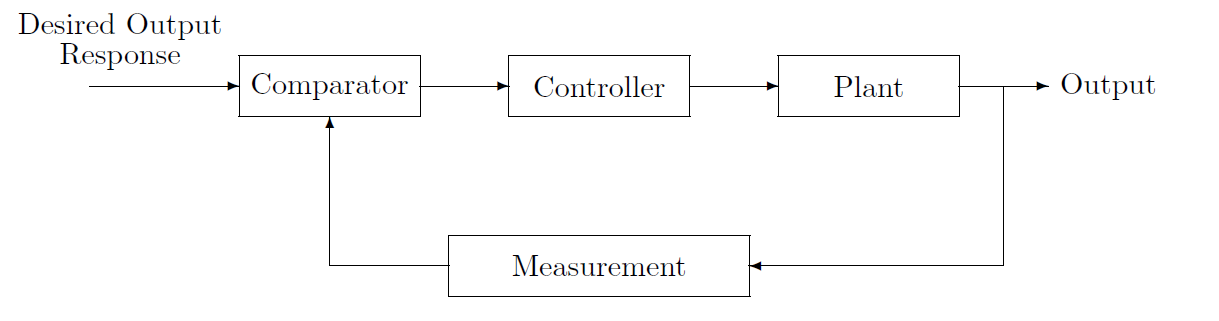
\includegraphics[width=0.75\textwidth]{figures/lab3_1.png}
        \caption{Closed-Loop Control System}
        \label{fig:bcg}
    \end{figure}
    \subsection{A Closed-Loop Feedback Model}
    {
        The block diagram of a generic closed-loop feedback control system is shown in Fig.1. In this figure, the “plant” is the system whose output we wish to control. A measurement is performed on the output by the measurement sub-system, which is then compared with the desired output, i.e., the input to the control system. The output of the comparator, which computes the difference between the desired and the actual output, is fed into a controller whose output serves as the input to the plant. If the comparator and measurement system were removed from the above diagram then one would be left with an open-loop (i.e., no feedback) controller.
    }
    \subsection{Closed-Loop Transfer Function}
    {
        As mentioned earlier, we will restrict our discussion to the case where all of the blocks shown in Fig.1 are LTI systems. Thus the input/output relationship of each of these blocks can be described by a system transfer function. Furthermore, we will realize the comparator as an adder and change the gain on the measurement to -1. With these changes, the block diagram of Fig. 2 becomes:
        \begin{figure}
            \centering
            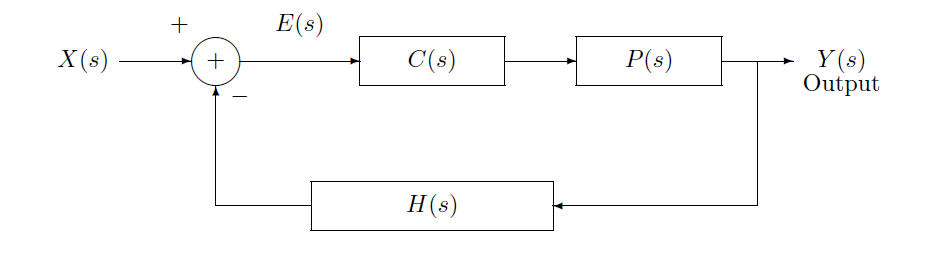
\includegraphics[width=0.75\textwidth]{figures/lab3_2.png}
            \caption{Closed-Loop Feedback Control System}
            \label{fig:lab3_2}
        \end{figure}
        It is a simple matter of algebra to compute the closed-loop transfer function, $G_{cl}(s) = Y(s)/X(s)$, of the systems shown in Fig.1 as indicated below.

        \begin{equation}
            Y(s) =E(s)C(s)P(s)
            \label{eq:eq1}
        \end{equation}

        \begin{equation}
            E(s)= X(s)-H(s)Y(s)
            \label{eq:eq2}
        \end{equation}

        Combining two equations above yields

        \begin{equation}
            G_{sl}(s)=\frac{Y(s)}{X(s)}=\frac{C(s)P(s)}{1+C(s)P(s)H(s)}
            \label{eq:eq3}
        \end{equation}
        
        \begin{equation}
            \frac{E(s)}{X(s)}=\frac{1}{1+C(s)P(s)H(s)}
            \label{eq:eq4}
        \end{equation}
    }
    
    \subsection{Examples of Feedback Control Systems}
    {
        \subsubsection{DC Motor Model}
        {
            Let's assume that we want to control the shaft position of a DC motor. To help design a controller for
            this DC motor, we mathematically model the angular position, $\theta (t)$ of the shift by the following differential equation
            \begin{equation}
                \frac{d^{2}\theta (t)}{dt^{2}} + \frac{d\theta (t)}{dt} = V(t),
                \label{eq:eq5}
            \end{equation}
            where V(t) is the voltage applied to the motor. Thus the plant is a LTI system that has the following system transfer function.

            \begin{equation}
                P(s) = \frac{1}{s(s+1)}
                \label{eq:eq6}
            \end{equation}
            This transfer function corresponds to a second-order LTI system with no zeros, and a pair of real poles located at the origin and at -1.
        }
        \subsubsection{No Controller}
        {
            Suppose we want the shaft of the motor to rotate by one radian per second by using a unit step as the input, $i.e., V(t) = u(t)$. Then

            \begin{equation}
                \theta(s)=V(s) P(s)=\frac{1}{s} \frac{1}{s(s+1)}=-\frac{1}{s}+\frac{1}{s^{2}}+\frac{1}{s+1}
                \label{eq:eq7}
            \end{equation}

            Consequently,

            \begin{equation}
                \theta(t)=\left(t-1+e^{-t}\right) u(t),
            \end{equation}

            which is clearly not going to achieve the desired rotation by one radian per second.

            \begin{figure}[H]
                \centering
                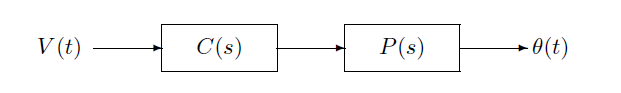
\includegraphics[width=0.75\textwidth]{figures/lab3_3.png}
                \caption{Open-Loop Controller.}
                \label{fig:lab3_3}
            \end{figure}

            i.e.,$C(s)=s$ of a unit-step input. Thus,
            \begin{equation}
                \theta(s)=V(s) C(s) P(s)=\frac{1}{s}\times \frac{1}{s(s+1)}=\frac{1}{s}-\frac{1}{s+1}
                \label{eq:eq8}
            \end{equation}
            Therefore, 
            \begin{equation}
                \theta(t)=\left(1-e^{-t}\right)u(t)
            \end{equation}
            Clearly, $lim_{t\rightarrow \infty} = 1$, so that this controller results in no steady-state error ($i.e., e(t) = V (t) − \theta (t) = 0\ as\ t\rightarrow \infty$) when the input is a unit step. The response of the DC motor to the unit step, however, is rather slow. It takes approximately 2.3 s for the shaft angle to reach $90\%$ of its final value of 1 radian.

            We might ask how well this same controller would work if the input were a ramp rather than a step. Under such circumstances
            \begin{equation}
                V(s) = \frac{1}{s}
            \end{equation}
            \begin{equation}
                \theta(s)=V(s) C(s) P(s)=\frac{1}{s^{2}}\times \frac{1}{s(s+1)}=-\frac{1}{s}+\frac{1}{s^{2}}+\frac{1}{s+1}
            \end{equation}
            Therefore,
            \begin{equation}
                \theta(t)=\left(t-1+e^{-t}\right) u(t)
            \end{equation}
            and the steady-state error is 1 radian/second. Thus the angular position of the shift deviates from the desired position by 1 radian as $t\rightarrow \infty$, and this differentiator-controller is inadequate for a ramp input.
        }

        \subsubsection{Sensitivity of an Open-Loop Controller to Plant Changes}
        {
            Suppose that overheating changes the transfer function of the motor by a small amount to become
            \begin{equation}
                P(s)=\frac{1}{(s+0.01)(s+1)}
            \end{equation}
            The step response of the motor now becomes
            \begin{equation}
                \theta(s)=V(s) C(s) P(s)=\frac{1}{s} s \frac{1}{(s+0.01)(s+1)}=\frac{100 / 99}{s+0.01}-\frac{100 / 99}{s+1}
            \end{equation}
            Therefore,
            \begin{equation}
                \theta(t)=(100 / 99)\left(e^{-0.01 t}-e^{-t}\right) u(t)
            \end{equation}
            and in steady state $lim_{t\rightarrow \infty=0}$, yielding a steady state error of one radian. This open-loop controller is quite sensitive to variations in the plant transfer function.

        }
            
        \subsubsection{Feedback (or Closed-Loop) Control}
        {
             Consider now the feedback control system shown in Fig. 2.2.1 with H(s) = 1, C(s) = Ks (i.e., a differential controller) and P(s) = 1/[s(s+1)] as before. Then according to Eq.3 the closed-loop transfer function is given by
            \begin{equation}
              G_{c l}(s)=\frac{Y(s)}{X(s)}=\frac{C(s) P(s)}{1+C(s) P(s) H(s)}=\frac{K s P(s)}{1+K s P(s)}=\frac{K}{s+(K+1)}
            \end{equation}
            and the step response becomes
            \begin{equation}
                \theta(s)=V(s) G_{c l}(s)=\frac{1}{s} \frac{K}{s+(K+1)}=\frac{K /(K+1)}{s}-\frac{K /(K+1)}{s+(K+1)}
            \end{equation}
            or equivalently,
            \begin{equation}
                \theta(t)=\frac{K}{K+1}\left(1-e^{-(K+1) t}\right) u(t)
            \end{equation}
            If K is sufficiently large, then the steady-state error, $lim_{t\rightarrow \infty}(V (t)-\theta (t)) = 1/(K + 1)$ will be small. Also note that the response time is much improved over that obtained by an open-loop controller.
        }

        \subsubsection{Sensitivity of the Closed-Loop Controller to Plant Changes}
       {
            As before we will consider the situation where the transfer function of the motor changes by a small amount to become that given by Eq.14. Using the same feedback controller described above, the closed-loop response becomes

            \begin{equation}
                G_{c l}(s)=\frac{K s}{s^{2}+(1.01+K) s+0.01}
            \end{equation}

            Thus the step response is given by

            \begin{equation}
                \theta(s)=\frac{K}{s^{2}+(1.01+K) s+0.01}=\frac{K /\left(a_{+}-a_{-}\right)}{s+a_{+}}-\frac{K /\left(a_{+}-a_{-}\right)}{s+a_{-}}
            \end{equation}

            where $$a_{\pm}=\frac{(1.01+K) \mp \sqrt{(1.01+K)^{2}-0.04}}{2}$$
            Therefore for K large $a_{+} \approx 0$ and $a_{-} \approx K$, yielding the step response 
            \begin{equation}
                \theta(t) \approx\left(1-e^{-K t}\right) u(t)
            \end{equation}
       }

       \subsubsection{Using Feedback to Stabilize Unstable Systems}
       {
           Consider a plant that has the following transfer function
            \begin{equation}
                P(s)=\frac{1}{s}
            \end{equation}
            This system is not BIBO stable, since its transfer function has a pole in the right-half plane. By implementing the feedback system shown in Fig.2, with $H(s) = 1$ and $C(s) = K$, the closed-loop transfer function becomes
            \begin{equation}
                G_{c l}(s)=\frac{C(s) P(s)}{1+C(s) P(s)}=\frac{1}{s+(K-1)}
            \end{equation}
            Thus for K > 1, the pole has been moved into the LHP and the system has become BIBO stable.
       }
    }
\section{Experimental Procedures}
{
    \subsection{Open Loop Control Plant}
    {
        \begin{enumerate}
            \item I construct the plant circuit according to Figure 4. Where $R_{0}= 10k\Omega,\ C_{1} = 100\mu F, C_{2} =0.22\mu F$.
            \item I set the A=1V, width=0.1s, f=1Hz to get impulse response.
            \item I set the A=1V, f=1Hz to get the step response.
        \end{enumerate}

        \begin{figure}[H]
            \centering
            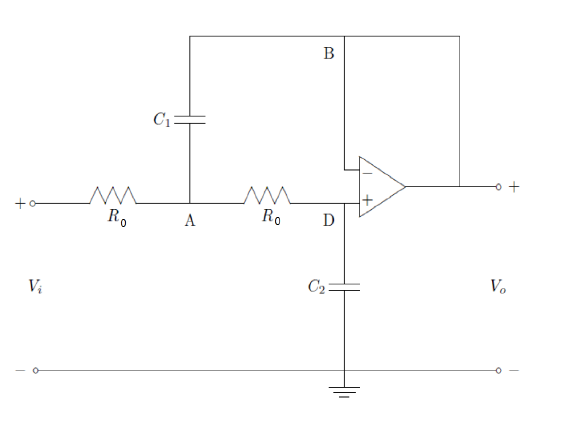
\includegraphics[width=0.45\textwidth]{figures/lab3_4.png}
            \caption{Plant Circuit.}
            \label{fig:lab3_4}
        \end{figure}
    }
    \subsection{Feedback Control}
    {
        \begin{enumerate}
            \item I add the feedback control circuit to the plant according to Figure 5. Where $R_{1}=R_{3}=150 k \Omega,\ R_{2}=3 k \Omega,\ C_{3}=0.47 \mu F$.
            \item I set A=1V, width=0.1s, f=1Hz to get the impulse response.
            \item I set the A=1V, f=1Hz to get the step response.
        \end{enumerate}
            
        \begin{figure}[H]
            \centering
            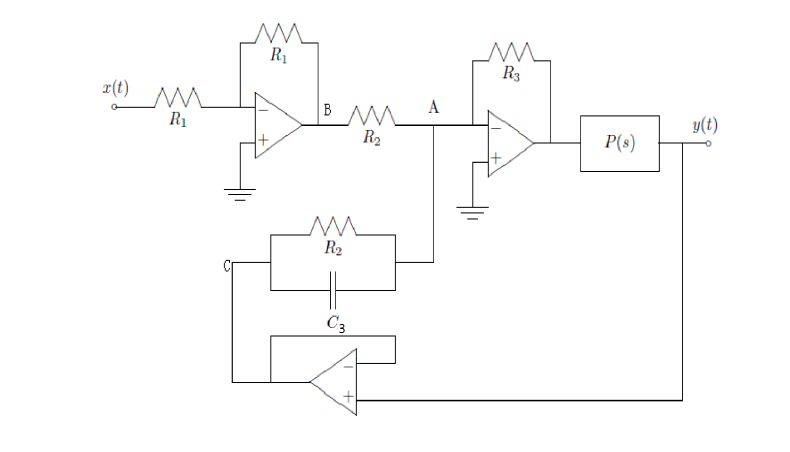
\includegraphics[width=0.75\textwidth]{figures/lab3_5.png}
            \caption{Feedback Control Circuit.}
            \label{fig:lab3_5}
        \end{figure}
            
    }
}

\section{Experimental Results}
{
    \subsection{Open Loop Control Plant}
    {
        \begin{figure}[H]
            \begin{small}
                \begin{center}
                    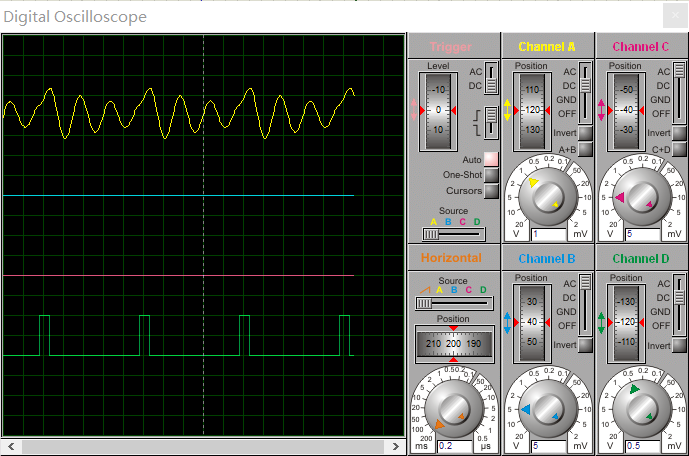
\includegraphics[width=0.45\textwidth]{figures/lab3_6.png}
                \end{center}
                \caption{Open Loop Control with the impulse response}
                \label{fig:lab3_6}
            \end{small}
        \end{figure}

        Then, we switch the input to the step function to get the simulation results.
        \begin{figure}[H]
            \begin{small}
                \begin{center}
                    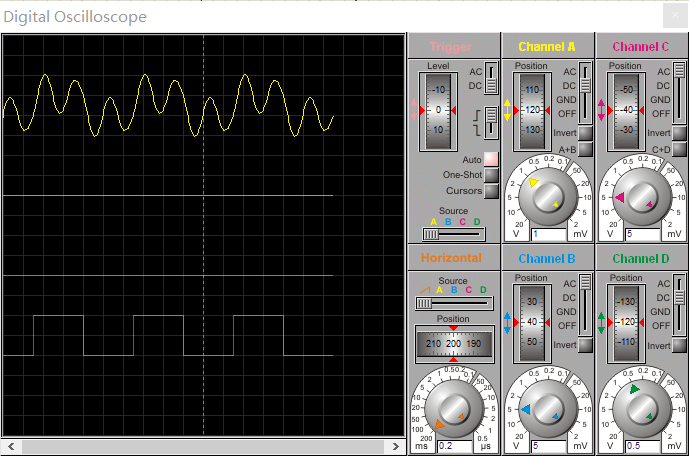
\includegraphics[width=0.45\textwidth]{figures/lab3_7.png}
                \end{center}
                \caption{Open Loop Control with the Step Response}
                \label{fig:lab3_7}
            \end{small}
        \end{figure}
    }
    \subsection{Feedback Control}
    {
        \begin{figure}[H]
            \begin{small}
                \begin{center}
                    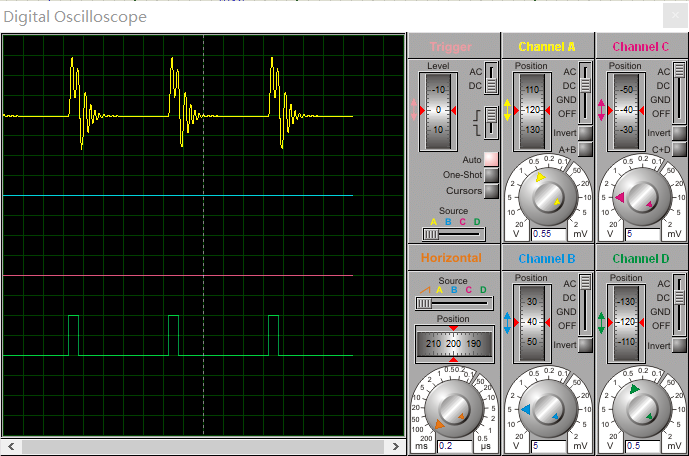
\includegraphics[width=0.45\textwidth]{figures/lab3_8.png}
                \end{center}
                \caption{Feedback Control With the Impulse Response}
                \label{fig:fig3_8}
            \end{small}
        \end{figure}
        Then, we switch the input to the step function to get the simulation results.
        \begin{figure}[H]
            \begin{small}
                \begin{center}
                    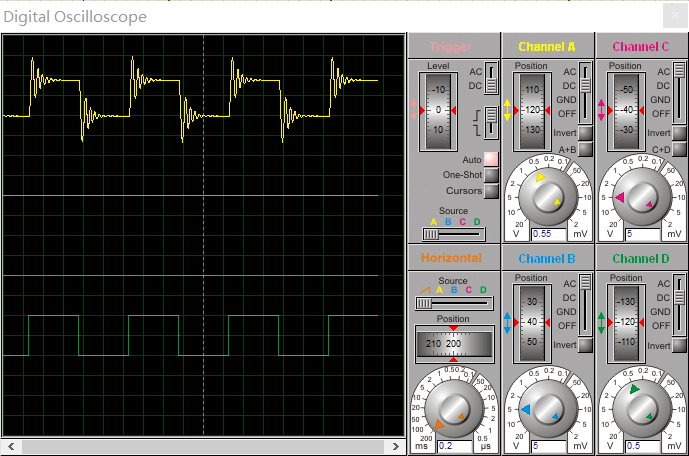
\includegraphics[width=0.45\textwidth]{figures/lab3_9.png}
                \end{center}
                \caption{Feedback Control with the Step Response}
                \label{fig:lab3_7}
            \end{small}
        \end{figure}
    }

}

\section{Discussion and Conclusion}
{
    \begin{enumerate}
        \item In the Open Loop Control part, we observes the difference of the input signal and the output. According to the experimental results, we find that they are quite close to each other. Thus, the slight difference can be ignored. We consider the difference may caused by the Gibbs Phenomenon. 
        \item In the Feedback Loop Control part, we also observes the difference of the input signal and the output. According to the experimental results, we find that they are quite close to each other. Thus, the slight difference can be ignored.
        \item By comparing the two different types of system, we find that the feedback system has a better performance of maintaining the stable output signal while the input is changing consistently.
    \end{enumerate}

    \textbf{Conclusion}:

        In this lab, I have learned the feedback control system via theoretical analysis and constructing actual circuit with op-amp. I also simulated the different types of circuits using Proteus. The result of our experiment are close to our expectation which are calculated theoretically. Also, by comparison, we find that the feedback control system would have a better performance when the input keeps changing. In all, I consider this lab as a successful one.
    }
}


\newpage
\section{Reference}
\begin{enumerate}
\item VE 216, "Spring 2020 Lab 3: Feedback Control Part I: Intro \& Pre-lab Assignment".  Available: \url{https://umjicanvas.com/courses/1527/files/folder/Lab}.
\end{enumerate}














\end{document}

